\chapter{The experiment by Purcell and Pound}
\label{ch:PandP}

CONTROLLARE PARALLELO O ANTIPARALLELO

The existence of negative absolute temperatures was first predicted by Lars Onsager in 1949 \cite{Onsager} in the context of 2D confined turbulence vortices. \\
The confinement of the vortices caused the phase space of the system to be bounded and Onsager showed that this results in a peak of the entropy as a function of the energy, in accordance
to what stated by the Ramsey's criterion. \\
The first experimental evidence of negative temperatures was the experiment carried by Purcell and Pound \cite{PandP} in 1951, who managed to bring the spins of a LiF crystal in a negative absolute temperatures 
state for several minutes.
In this section I want to illustrate the experimental procedure followed by Purcell and Pound to realize such a state.\\

The experiment used a system of nuclear spins on a LiF crystal lattice immersed in a uniform magnetic field $\ve h$.
The energy of the system is given by the analogous of equation \ref{eq:Hamiltonian_lattice_spin}
\begin{equation*}
    E = - \ve h \cdot \ve M + \mathcal{H}_{ss} + \mathcal{H}_{sl}
\end{equation*}
where $\ve M$ is the magnetic moment vector $\ve M = g \frac{q}{2m} \, \ve S$, $\ve S$ is the spin and $g$ is the Landé factor. \\
As before we consider negligible the spin-spin interaction term but still considering it non-zero since it is fundamental for keeping the system in internal equilibrium \cite{main_article}. \\
The spin-lattice interaction is characterized by the typical relaxation time $\tau_{L}$ which was found to be around 5 minutes for the considered system. For times much smaller than $\tau_L$, 
the system can be considered as in a transient equilibrium, and the particle's states distribution defines a spin temperature according to equation \ref{eq:spin_temperature}. This temperature is precisely the one
that was deduced to be negative. The effective energy for the system for the experiment was then 
\begin{equation}
    E \approx - \ve h \cdot \ve M
    \label{eq:energy_PandP}
\end{equation}\\
Initially the system was brought into equilibrium aligning all the spins with the magnetic field in either a parallel or antiparallel way: for positive temperatures, for what said in chapter \ref{ch:TLS}, we expect the majority of the spins to be parallel causing the energy given by 
equation \ref{eq:energy_PandP} to be negative. \\
Then, suddently, the magnetic field is switched in direction, causing the majority of the spins to be antiparallel to the magnetic field, hence giving raise to a positive energy. This state is characterized by a negative spin temperature.
Figure \ref{fig:PandP_switch} illustrates the effect of the magnetic field making use of the entropy-energyrelation given by equation \ref{eq:entropy_E_TLS}.
\begin{figure}
    \centering 
    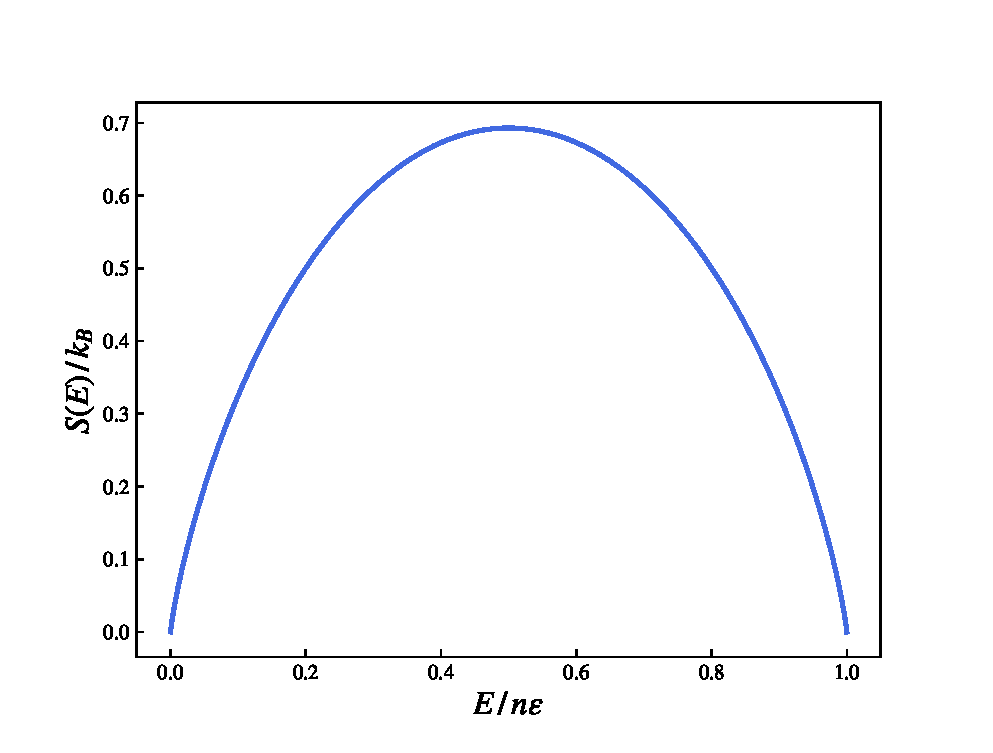
\includegraphics[scale=0.5]{./images/entropy_TLS}
    \caption{}
    \label{fig:PandP_switch}
\end{figure}
\begin{figure}[htbp]
    \centering 
    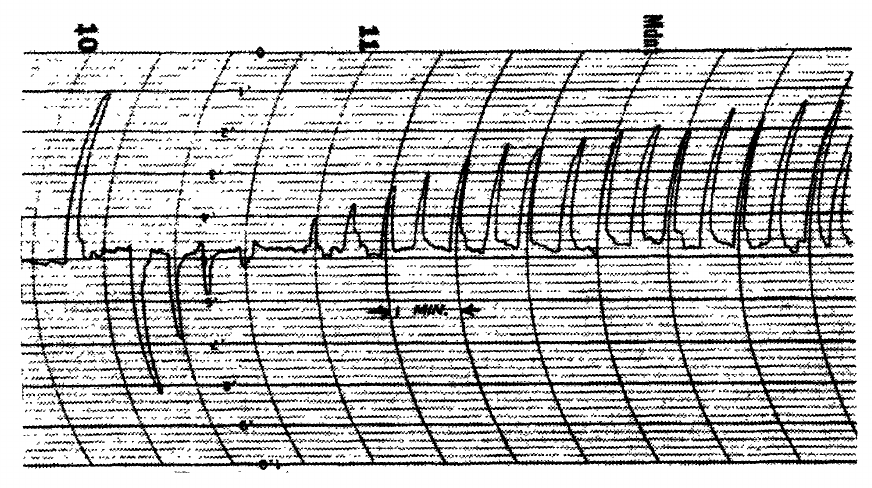
\includegraphics[scale=0.5]{./images/PurcellPound.png}
    \caption{The plot (adapted from \cite{PandP}) reports the record of the nuclear magnetization during the experiment. The first peak denotes
    the initial equilibrium state in which the spins are aligned with the magnetic field in the lowest energy state. As the magnetic field is istantaneously reversed,
    the spins remained aligned in the opposite direction of the field, remaining in the highest enery state and causing the second (negative) peak. After a relaxation time
    $\tau_L$ the spin system returns in equilibrium in the lowest energy state.}
    \label{fig:PandP}
\end{figure}